\documentclass[10pt]{exam}
\usepackage[phy]{template-for-exam}
\usepackage{multirow}
\usepackage[table,dvipsnames]{xcolor}
\usepackage{pgf-pie}
\usepackage{wrapfig}
\usepackage{enumitem}
\usepackage{graphicx}
\graphicspath{{./images}}
\setlist[enumerate]{topsep=0pt,itemsep=-1ex,partopsep=1ex,parsep=1ex}
\usepackage[super]{nth}


\newcommand{\mg}{\rowcolor{Goldenrod}}


\title{Course Information Guide \\ Physics I}
\author{Rohrbach}


\begin{document}

\maketitle

\noindent Zachary J. Rohrbach, Instructor

\noindent (317) 544-5000 x5131

\noindent \texttt{ZJRohrbach@avon-schools.org}

\section*{Course Description}

Physics is the study of how the universe works on the most fundamental level.  In this 
class, you will use your powers of observation and logical as well as mathematical 
reasoning to describe, explain, and predict the behavior of objects.

\paragraph{Course Goals} 
As a result of taking Physics I, you will:

\begin{enumerate}
	\item Know and understand the process that is used to make the scientific discoveries that 
				are reported in the media or in the workplace
	\item Understand the scientific principles that underlie motion, forces, waves, and electricity.
	\item Apply your mathematical skills to solving real-world problems
	\item Develop problem solving and scientific literacy skills
\end{enumerate}


\section*{Classroom Expectations}

\begin{center}
  \begin{tabular}
    {
      p{.15\textwidth}
      p{.03\textwidth}
      p{.7\textwidth}
		}
		
    \hline
      \mg \bf Accountable 
      			&  1. & Start the period with your {\bf calculator}, 
                  {\bf notebook}, and {\bf reading book} on your 
                  desk.
      \\
      \mg   &  2. & Bring your {\bf computer} and {\bf charger} with you
                  every day.
      \\
      \mg 	&  3. & Take care of restroom breaks outside of 
                  class.
                  \vspace{-1em}
                  \begin{quotation}
                  	\noindent\small
										\textit{In the} rare \textit{event that you’d need to use the restroom 
										during class, I will only fill out a pass in your own agenda.  Also, I will 
										only do this a maximum of once per week.}
										\vspace{-1.5em}
                  \end{quotation}

      \\
     	\mg   &  4. & Be in the classroom by the time the bell 
                  rings.
                  \vspace{-1em}
                  \begin{quotation}
                  	\noindent\small
										\textit{My tardy policy is the same as the school’s. You are tardy if you 
										are not in the classroom by the time the bell rings.  You will be given 
										a detention on your \nth{3} and \nth{4} tardies and referred to Saturday School 
										for \nth{5} and \nth{6} tardies.}
										\vspace{-1.5em}
                  \end{quotation}
      \\  
    
    \hline
    \bf Respectful
          &  5. & SSR time is for silent reading.
                 	\vspace{-1em}
                  \begin{quotation}
                  	\noindent\small
										\textit{We will have 10-15 minutes of sustained silent reading (SSR) 
										at the beginning of the period.  Why do we do silent reading in a 
										science class?  Research shows that people who read do better in 
										school and have lower levels of stress.  It also is an opportunity to 
										take a breath and set the tone for the class period.}
										\vspace{-1.5em}
                  \end{quotation}
          \\   
          &  6. & Quietly listen to the speaker.         
          \\  

    \hline
      \mg \bf Engaged
      		&  7. & Keep phones and earbuds put away.
                  \vspace{-1em}
                  \begin{quotation}
                  	\noindent\small
										\textit{If I see a phone or earbuds, I will ask you to put them in 
										a paper bag and staple it shut. This bag will stay on your desk for 
										the rest of the period.  It must stay shut until the bell to end class
										rings.  If you fail to comply with this, you will be given a detention.}
										\vspace{-1.5em}
                  \end{quotation}
      \\
      \mg &  8. & When you are finished with your work, 
                  you may read a book.
      \\
      \mg &  9. & Stay engaged and working until the 
                  {\bf two-minute alarm}.
      \\
      \mg & 10. & Persevere through difficult problems.
      \\  

    \hline
  \end{tabular}
\end{center}

\pagebreak

\section*{Required Materials}

You are expected to bring the following materials with you to class every day.  

\begin{center}

\begin{tikzpicture}
	
	
	\node [font=\large] at (0, .5) {Notebook};
	\node [font=\small\it] at (0, 0)  {(will be provided to you)};
	\node at (0,1.7) {
\includegraphics[width=2.4cm]{notebook}};


	\node [font=\large] at (3, .5) {Reading};
	\node [font=\large] at (3, 0)  {Book};
	\node at (3,1.7) {
\includegraphics[width=2.4cm]{book}};


	\node [font=\large] at (6, .5) {Charged};
	\node [font=\large] at (6, 0)  {Laptop};
	\node at (6,1.7) {
\includegraphics[width=2.4cm]{laptop}};

	
	\node [font=\large] at (9, .5) {Computer};
	\node [font=\large] at (9, 0)  {Charger};
	\node at (9,1.7) {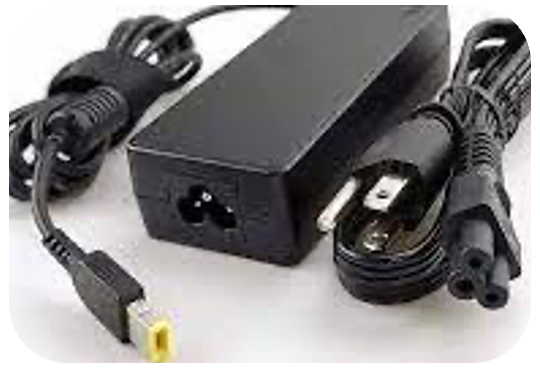
\includegraphics[width=2.4cm]{charger}};
	
	\node [font=\large] at (12, .5) {Student};
	\node [font=\large] at (12, 0) 	{Agenda};
	\node at (12,1.7) {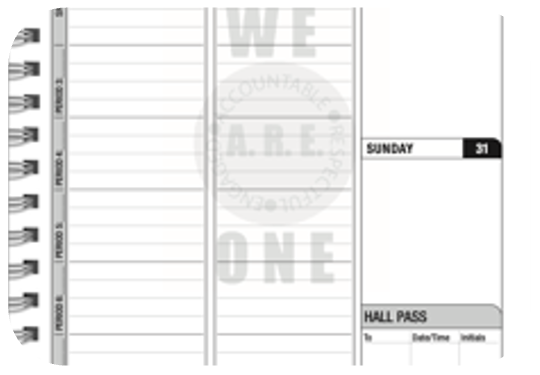
\includegraphics[width=2.4cm]{agenda}};


\end{tikzpicture}

\end{center}




\section*{Methods of Evaluation}

Your pre-exam grade will be based on the methods of 
evaluation shown below. The weighting of each of these 
categories is subject to change. Your overall class 
grade will consist of the pre-exam grade (85\%) and the
final exam grade (15\%).

\begin{center}
	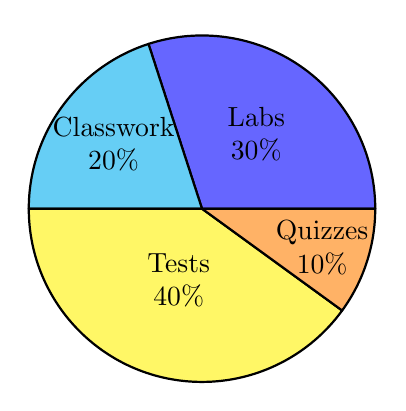
\begin{tikzpicture}
		\pie[text=inside, radius=2.2]{
			30/Labs,
			20/Classwork,
			40/Tests,
			10/Quizzes
		}
	\end{tikzpicture}
\end{center}

Tests may be corrected for half credit back on missed 
questions.  Test corrections are due by midterm.  In other 
words, test corrections for units completed before the 
midterm will not be accepted after the midterm.  Directions 
on how to do corrections will be given later.



\section*{Other Class Policies}

\paragraph{Late Work}
	Deadlines for assignments will be announced in class and posted on Schoology.  Late work 
	is subject to a 50\% penalty.  Late work for a particular unit will not be accepted after
	the test is given for that unit.

\paragraph{Absences and Makeup Work}
	Mr. Rohrbach will often also post additional video explanations and recordings on Schoology for
	students who are absent.  If you are absent, it is your responsibility to check Schoology and
	contact Mr. Rohrbach with any questions.  Because of the resources on Schoology, you should not
	assume that you will be given extensions because you were absent. If you find you will need an
	extension, you should contact Mr. Rohrbach before you come back to school. 

\paragraph{Contacting Mr. Rohrbach}
	Parents and students should feel free to contact Mr. Rohrbach at any time via email 
	(\texttt{ZJRohrbach@avon-schools.org}), phone (317-544-5000 x5131), \mbox{ParentSquare}, 
	or Schoology.




\end{document}